\documentclass{article}
\usepackage{tikz}
\usetikzlibrary{datavisualization}
\usetikzlibrary{datavisualization.formats.functions}
\pagestyle{empty}

\begin{document}
\colorbox{white}{%
    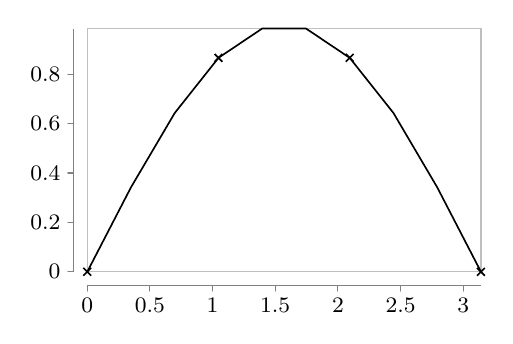
\begin{tikzpicture}
        % ��ѧ
        \datavisualization [scientific axes=clean, visualize as line=my data, my data={style={mark=x, mark repeat=3}}]
            data [format=function] {
                var x : interval [0:pi] samples 10;
                func y = sin(\value x r);
            };
    \end{tikzpicture}
}
\end{document} 